\documentclass[a4paper, 12pt]{article}
\usepackage[toc,page]{appendix}
\usepackage{graphicx}
\usepackage{float}
\usepackage{pdfpages}
\usepackage{url}
\usepackage[margin=1.25in]{geometry}
\usepackage{hyperref}
\hypersetup{
	colorlinks,
	citecolor=green,
	filecolor=black,
	linkcolor=black,
	urlcolor=blue
}

%opening
\title{{\Huge Distributed Systems Project} \\ \vspace{3mm}
	{\LARGE Simulate message delivery guarantees such as FIFO and Arbitrary, and their impact on some Mutual Exclusion Distributed Algorithm }  \\ \vspace{4mm}
}
\author{Ankit Pant  2018201035 \\ 
	Harshita Agrawal 2018201014 \\
	Ravi Jakhania 2018201018 }
\date{Submitted on: \today}

\begin{document}
	\maketitle
	\thispagestyle{empty}
	\newpage
	\pagenumbering{roman}
	\tableofcontents
	\newpage
	
	\setcounter{page}{1}
	\pagenumbering{arabic}
	\section{Introduction}
		Distributed systems are quite ubiquitous these days owing to the large amounts of data that is being generated and processed. It is essential that when the computing infrastructure is distributed, the communication between these components is robust. Though the advancement in hardware and network technologies have made large scale distributed systems possible, we still need a layer of dependable software systems that makes reliable communication possible between the distributed system and help manage the various components. Since various systems are communicating with each other and may be accessing some common resources, it is also imperative that we have some algorithms in place that prevent more than one system from accessing the critical resource at a time and prevent race conditions. We do this by using Distributed Mutual Exclusion Algorithms.
		\par This project aims to explore and simulate two modes or channels of communication i.e. First In First Out or \emph{FIFO} channels and \emph{Arbitrary} channels. A more detailed description of them are presented in the following sections. After the implementation of the \emph{FIFO} and \emph{Arbitrary} channels, we simulate a Distributed Mutual Exclusion Algorithm known as the Lamport's Mutual Exclusion Algorithm on the channels and measure the impact of the communication channels on the distributed mutual exclusion algorithm.
		\par The following sections elaborate more on the literature as well as describe the methodology as well as the experimental setup and results obtained. The report ends by reporting on the conclusions and suggesting improvements as future scope.
		
	\section{Literature Review}
		This section theoretically elaborates on the various terms and components of the project. This section also delves into the components of the distributed systems that have been used to complete the project. Each such component is elaborated in the following subsections:
		
		\subsection{Message Ordering and Group Communication}
			The importance of group communication cannot be over-stated in distributed systems. In most scenarios, a node is able to communicate with all other nodes that are part of the distributed system. Apart from the aspect of nodes being able to communicate with each other, the order in which the messages are delivered is also important  as it determines the order of execution of commands and also helps to keep the system consistent. There are several such message orderings, a few of which are elaborated in the following subsections.
			
			\subsubsection{Arbitrary Order}
				Arbitrary order implies that there is no ordering between messages sent by one node to the other. This message ordering is also called \emph{non-FIFO} ordering. For example if a process `P1' sends two messages (m1 and m2) to `P2' and the timestamp of message \textit{m1} is \textit{t1} and for message \textit{m2} is \textit{t2} where $t1<t2$ the process `P2' may either receive message \textit{m1} before message \textit{m2} or it may receive message \textit{m2} before message \textit{m1}.
				
			\subsubsection{FIFO Order}
				FIFO order or First In First Out ordering implies that if messages are sent by a process to another process in a particular order, they are received by the other process in the same order that they were sent \cite{1}. For instance if a process `P1' sends two messages (m1 and m2) to `P2' and the timestamp of message \textit{m1} is \textit{t1} and for message \textit{m2} is \textit{t2} where $t1<t2$ the process `P2' must necessarily receive message \textit{m1} before message \textit{m2}. In this message ordering it is ensured that multicast from each sender are received in the order they are sent, at all receivers. The relative ordering between multicast messages from different senders is not important.
				
			\subsubsection{Causal Ordering}
				In causal ordering implies that if two send (or more) events happen then their corresponding receive events happen in the same order as well throughout the distributed system. It is a stricter version of \textit{FIFO} ordering and the relative ordering between multicast messages from different senders is also taken into account. Thus for example if there are two messages \textit{m1} and \textit{m2} then if send timestamp(\textit{m1}) $<$ send timestamp(\textit{m2}), then for each destination of those messages, receive timestamp(\textit{m1}) $<$ receive timestamp(\textit{m2}) \cite{2}.
							
				
		\subsection{Distributed Mutual Exclusion Algorithms}
			Mutual exclusion is one of the core problems when running distributed systems. It needs to be ensured that more than two nodes are not modifying the same object and not creating race conditions. Thus, mutual exclusion states that only one process must be executing its critical section at a given point in time. Since there is no traditional notion of shared memory in distributed systems, the solutions like semaphores cannot be used. Hence it results in a need to implement distributed mutual exclusion algorithms. Distributed mutual exclusion algorithms are implemented using these basic approaches \cite{3}:
			\begin{itemize}
				\item Token based approach
				\item Non-token based approach
				\item Quorum based approach
			\end{itemize}
			The following sub sub-section briefly discusses a token based distributed mutual exclusion algorithm which has been simulated in this project.
			
			\subsubsection{Lamport's algorithm}
				Lamport's algorithm is a Token based Distributed Mutual Exclusion algorithm. This algorithm executes the critical section requests from various processes in the increasing order of timestamps. Every node is also required to keep a queue called the \textit{request queue} which stores the critical section requests in the increasing order of timestamps. However it is required that the channel delivers messages in \textit{FIFO} order for this algorithm to execute correctly. The algorithm has three phases \cite{4} namely:
				\begin{itemize}
					\item Requesting the critical section
					\item Executing the critical section
					\item Releasing the critical section
				\end{itemize}
			
				The following diagram \ref{Lamportalgo} provides the pseudocode for the algorithm.
				
				\begin{figure}[H]
					\label{Lamportalgo}
					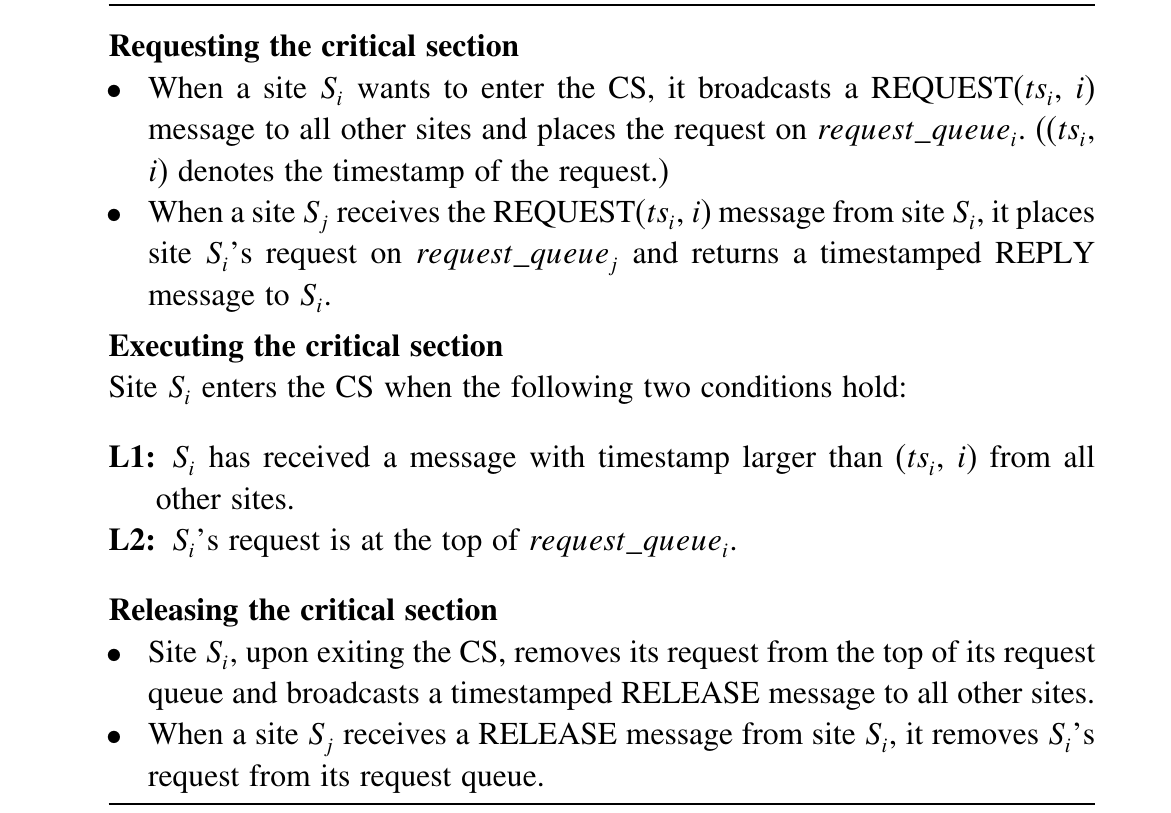
\includegraphics[width=\linewidth]{lamport_algo.png}
					\caption{Pseudocode for Lamport's Algorithm \cite{4}}
				\end{figure}
			
				
	\section{Methodology}
			This sections describes the methodology of the project. First and foremost, two message ordering modes were created, namely \textit{FIFO} and \textit{Arbitrary}. After creating these message ordering modes, Lamport's Algorithm was run on top of the channels preserving the \textit{FIFO} and \textit{Arbitrary} message ordering respectively. Using the Lamport's Algorithm, a dummy \textit{critical section} of each node was run and it was ensured that only one node can execute its critical section at one time and the order of execution is based on the timestamp of request to execute critical with the lowest timestamp given the highest priority.
			\par The performance of the algorithm was then examined by running it on both the message ordering modes and the impact of the message ordering mode was measured on the algorithm, primarily based on the correctness. The following sub-sections elaborate on the various aspects of the project.
			
			
		\subsection{System Model}
			To run the simulation we assume a distributed system with six nodes. It is also assumed that all nodes are non-Byzantine. Since the channel is reliable, message delivery guarantee is ensured and if a node communicates with any other node, it is guaranteed that the other node will receive the message. Each node is fully capable to send and receive messages as well as request (to execute) the critical section. Each node is also capable of communicating with every other node as this is also one of the pre-requisites of the Lamport's Algorithm. The implementation also handles arbitrary node (channel) failure by using a timeout mechanism.
			
		\subsection{Development Environment}
			The project was developed in python and a bash script was written to run the various nodes. Multithreading was used to manage asynchronous sends and receives.  The distributed system so created was tested in bash terminal where each node used the IP address of \textit{localhost} with different \textit{port numbers}.
			
		\subsection{Creating FIFO Ordered Channel}
			The FIFO ordered channel was created using TCP connections for maintaining reliability and message delivery guarantee. Each node has a send and receive method (with helper functions) to be able to send messages to other nodes and receive messages from other nodes respectively.
			
		\subsection{Creating Arbitrary Ordered Channel}
			Arbitrary channels were simulated by adding a random delay while sending each message. This effectively simulated out of order delivery to the recipient node. This channel also has TCP as the underlying protocol to ensure reliability and message delivery guarantee.
			
		\subsection{Implementing Lamport's Algorithm}
			Lamport's algorithm was implemented such that it may run on each of the ordered channels. As required by the algorithm each node maintains a priority queue in which all critical section requests are stored in increasing order of timestamps. Each node also maintains a local clock for timestamping purposes. The three types of messages, \textit{Request},\textit{Reply}, and \textit{Release} (which are vital to the algorithm) are also exchanged as required.
			
		\subsection{Testing}
			The testing phase consists of three sub-parts namely testing the FIFO ordered channel, testing the Arbitrary ordered channel, and testing mutual exclusion algorithm on both the ordered channels. A driver program is written that gives a menu-based interface to run either of the test cases. The test cases are written out in \textit{csv} files that makes it easy to test variety of situations without having to hard-code the test cases. 
			
	\section{Experimentation and Results}
		The test cases were run using the \textit{Test.sh} bash script that starts all nodes in the Distributed System and gives a menu-based choice on which test to run. The inputs were taken from the \textit{Check\_channel.csv} file to test the \textit{FIFO} ordered and \textit{Arbitrary} ordered channels, and from the \textit{ME\_Test.csv} file to run the Lamport's mutual exclusion algorithm on both channels consecutively.
		\subsection{Testing the Message Ordering}
			The \textit{FIFO} and \textit{Arbitrary} Ordered channels created, were tested and were found to run correctly. Messages send from a process to another are received in the same order they were sent for the \textit{FIFO} ordered channel. Messages sent by a process through the \textit{Arbitrary} channel were received arbitrarily as expected. The results were written to two separate files, \textit{FIFO\_Result.txt} and \textit{Arbitrary\_Result.txt} respectively. Figure \ref{ChannelTest} shows the sample test file, while Figures \ref{FIFORes} and Figure \ref{AribraryRes} show the output of the test file on \textit{FIFO} ordered and \textit{Arbitrary} ordered channels respectively. The test file has comma separated entries where in each row the first entry corresponds to sender node, the second entry corresponds to the receiver node and the third entry corresponds to the message.
			
			\begin{figure}[H]
				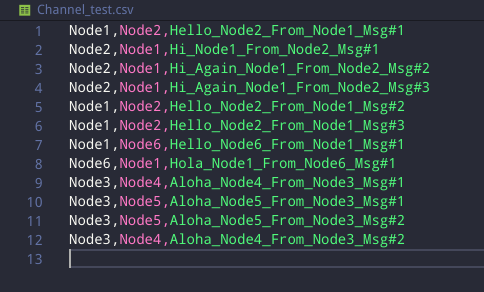
\includegraphics[width=\linewidth]{Channel_Test.png}
				\caption{A sample test file}
				\label{ChannelTest}
			\end{figure}
		
			\begin{figure}[H]
				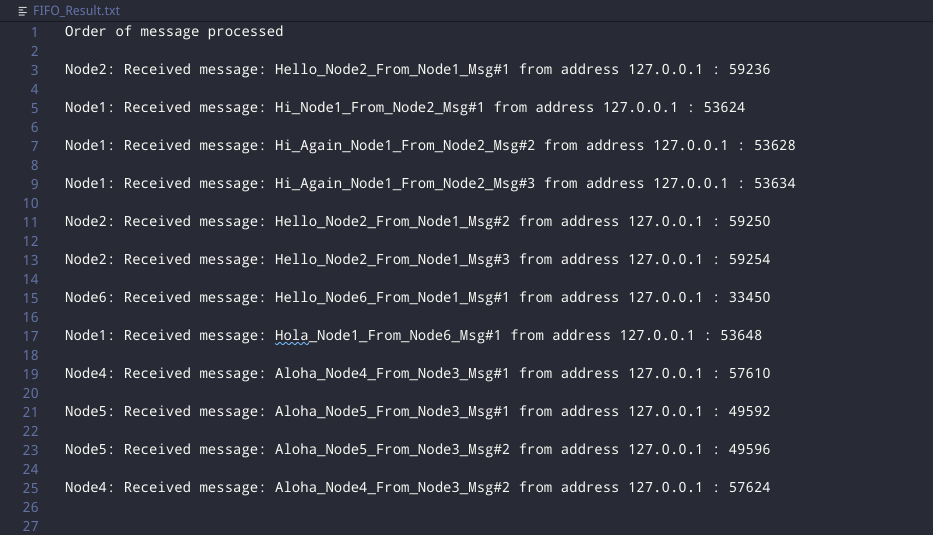
\includegraphics[width=\linewidth]{FIFO_Res.png}
				\caption{Output on FIFO ordered channel for the test file}
				\label{FIFORes}
			\end{figure}
		
			\begin{figure}[H]
				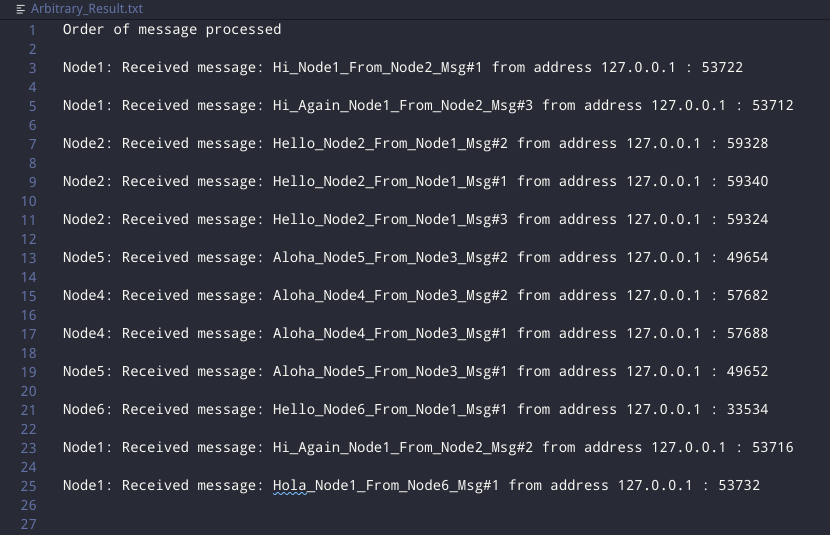
\includegraphics[width=\linewidth]{Arbitrary_Res.png}
				\caption{Output on Arbitrary ordered channel for the test file}
				\label{AribraryRes}
			\end{figure}
			
			Hence it can be seen from the figures above that the channels work as expected.
			
		\subsection{Testing Mutual Exclusion Algorithm}
			The Lamport's algorithm was then run on both \textit{FIFO} ordered channel and \textit{Arbitrary} ordered channel and found to give correct result for the \textit{FIFO} ordered channel. For the \textit{Arbitrary} ordered channel, Lamport's Algorithm fails as was expected and more than one process succeeds in securing the critical section since the messages are not delivered in FIFO order. The output of the algorithm was written to the file \textit{Mutual\_Execlusion\_Result.txt}. Figure \ref{METest} shows the sample test file while the figure \ref{MEResF} and \ref{MEResA} show the output corresponding to running the algorithm in \textit{FIFO}  ordered channel and arbitrary ordered channel respectively. The test file stores the order in which the nodes should execute the critical section. 
			
			\begin{figure}[H]
				\centering
					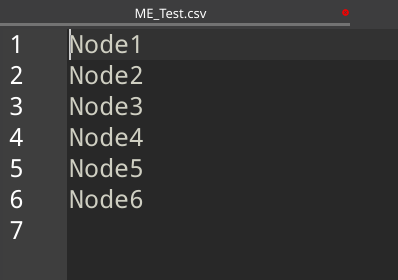
\includegraphics[width=60mm]{ME_Test.png}
					\caption{A sample test file}
					\label{METest}
			\end{figure}
		
			\begin{figure}[H]
				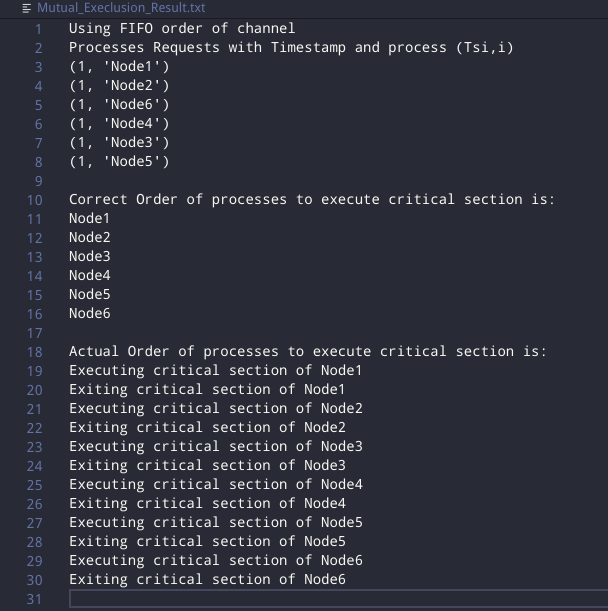
\includegraphics[width=\linewidth]{ME_FIFO.png}
				\caption{Output on FIFO ordered channel for the test file}
				\label{MEResF}
			\end{figure}
		
				\begin{figure}[H]
				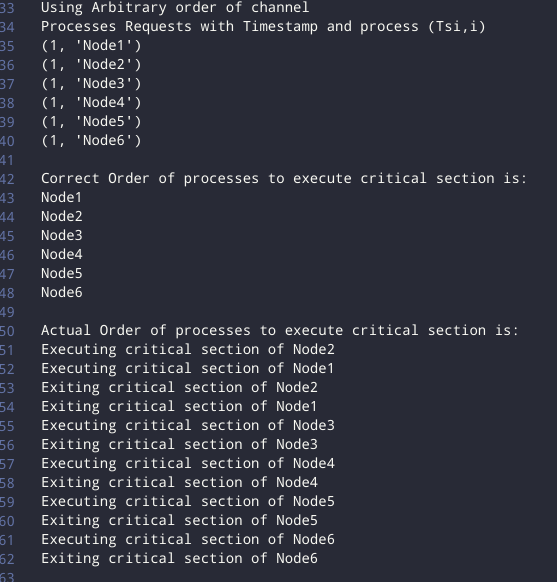
\includegraphics[width=\linewidth]{ME_Arbitrary.png}
				\caption{Output on Arbitrary ordered channel for the test file}
				\label{MEResA}
			\end{figure}
		
		Hence through the figures above it can be seen that when Lamport's Algorithm is run for \textit{FIFO} ordered channel, it produces the correct output. However the algorithm fails when it is run on an \textit{Arbitrary} Ordered Channel.
		
		\subsection{Impact of Channel on Mutual Exclusion Algorithm}
			This sub-section describes the impact of running the Distributed Mutual Exclusion Algorithm (Lamport's Algorithm) on \textit{FIFO} ordered and \textit{Arbitrary} ordered channels.
			
			\subsubsection{Correctness}
				Correctness of the algorithm running on the two channels is compared. Since Lamport's Algorithm necessarily requires a \textit{FIFO} ordered channel for its correct execution, it does not run correctly on running in in an \textit{Arbitary} ordered channel.\\
				\indent \textbf{FIFO Ordered Channel:} Algorithm runs correctly. \\
				\indent \textbf{Arbitrary Ordered Channel:} Algorithm fails.
			
			\subsubsection{Number of Messages}
				Number of messages exchanged when running on the two channels is compared. Since execution is done on reliable channels (using TCP), we see no difference in the number of messages exchanged.\\
				\indent \textbf{FIFO Ordered Channel:} $3(N-1)$. \\
				\indent \textbf{Arbitrary Ordered Channel:} $3(N-1)$.
				
			\subsubsection{Algorithmic Runtime}
				Since the communication between nodes in the distribution system can have uncertain delays (in spite of guaranteed message delivery), the total runtime of executing Lamport's algorithm on either channel was not measured as it was not well understood how to eliminate the effect of random network delays while running the algorithm.
		
	\section{Conclusion}
		It is necessary for a distributed system to have mutual exclusion for its proper functioning. The ordering of messages in channels connecting the nodes also play a critical part in supporting the algorithms that can be run on the system. Through this project, two such message ordering channels, namely \textit{FIFO} ordered and \textit{Arbitrary} ordered channels were explored. The channels were simulated and after that a distributed mutual exclusion algorithm (Lamport's algorithm) was run on them to measure the impact of message ordering on the algorithm.
		\par It was found that the ordering in channels have a significant impact on Lamport's Mutual Exclusion algorithm and while \textit{FIFO} ordered channels runs the algorithm without a problem, \textit{Arbitrary} ordered channel can cause the algorithm to fail. Hence through this project, we conclude that Lamport's Mutual Exclusion algorithm requires (at least) a \textit{FIFO} ordered channel and it may fail if we cannot guarantee the First In First Out message ordering.
		
	\section{Future Scope}
		Currently Lamport's algorithm fails for \textit{Arbitrary} ordered channels. The modifications can be made to have Lamport's algorithm run on \textit{Arbitrary} ordered channels too. Resolution may be done by:
		\begin{itemize}
			\item Adding buffer at receivers
			\item Buffer orders messages correctly by timestamp
			\item After all messages are received and correctly ordered, forward them to the mutual exclusion algorithm
		\end{itemize}
	
	\begin{thebibliography}{4}
		\bibitem{1} \textit{FIFO executions}, Ajay D. Kshemkalyani \& Mukesh Singhal, Page 191, Distributed Computing Principles, Algorithms, and Systems.
		\bibitem{2} \textit{Causally ordered (CO) executions}, Ajay D. Kshemkalyani \& Mukesh Singhal, Page 191, Distributed Computing Principles, Algorithms, and Systems.
		\bibitem{3}\textit{Distributed mutual exclusion algorithms}, Ajay D. Kshemkalyani \& Mukesh Singhal, Page 305, Distributed Computing Principles, Algorithms, and Systems.
		\bibitem{4}\textit{Lamport's Algorithm}, Ajay D. Kshemkalyani \& Mukesh Singhal, Page 309, Distributed Computing Principles, Algorithms, and Systems.
	\end{thebibliography}
			
\end{document}
 